
\begin{figure}[H]
  {
    \setlength{\tabcolsep}{3.0pt}
    \setlength\cmidrulewidth{\heavyrulewidth} % Make cmidrule = 
    \begin{adjustbox}{height=5cm,center}
      \footnotesize
      \begin{tabular}{ll}

        \makecell[l]{
\icode{.BYTE \$FF,\$01,\$01,\$FF}\\
\icode{.BYTE \$FF,\$FF,\$01,\$01}
} & \makecell[l]{

\includegraphics[width=1.3cm]{src/colorspace_patterns/pixels/pixel_pattern5_2.png}%

\includegraphics[width=1.3cm]{src/colorspace_patterns/pixels/pixel_pattern5_3.png}%
} \\
        \midrule

        \makecell[l]{
\icode{.BYTE \$FE,\$02,\$02,\$FE}\\
\icode{.BYTE \$FE,\$FE,\$02,\$02}
} & \makecell[l]{

\includegraphics[width=1.3cm]{src/colorspace_patterns/pixels/pixel_pattern5_4.png}%

\includegraphics[width=1.3cm]{src/colorspace_patterns/pixels/pixel_pattern5_5.png}%

\includegraphics[width=1.3cm]{src/colorspace_patterns/pixels/pixel_pattern5_6.png}%

\includegraphics[width=1.3cm]{src/colorspace_patterns/pixels/pixel_pattern5_7.png}%
} \\
        \midrule

        \makecell[l]{
\icode{.BYTE \$FD,\$FF,\$01,\$03,\$03,\$01,\$FF,\$FD}\\
\icode{.BYTE \$FF,\$FD,\$FD,\$FF,\$01,\$03,\$03,\$01}
} & \makecell[l]{

\includegraphics[width=1.3cm]{src/colorspace_patterns/pixels/pixel_pattern5_8.png}%
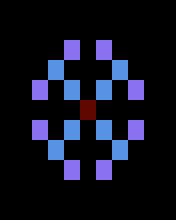
\includegraphics[width=1.3cm]{src/colorspace_patterns/pixels/pixel_pattern5_9.png}%

\includegraphics[width=1.3cm]{src/colorspace_patterns/pixels/pixel_pattern5_10.png}%

\includegraphics[width=1.3cm]{src/colorspace_patterns/pixels/pixel_pattern5_11.png}%

\includegraphics[width=1.3cm]{src/colorspace_patterns/pixels/pixel_pattern5_12.png}%
} \\
        \midrule

        \makecell[l]{
\icode{.BYTE \$FD,\$03,\$03,\$FD}\\
\icode{.BYTE \$FD,\$FD,\$03,\$03}
} & \makecell[l]{
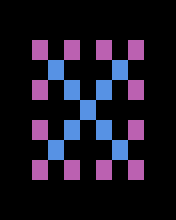
\includegraphics[width=1.3cm]{src/colorspace_patterns/pixels/pixel_pattern5_13.png}%
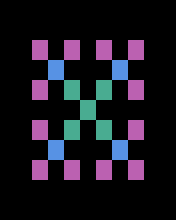
\includegraphics[width=1.3cm]{src/colorspace_patterns/pixels/pixel_pattern5_14.png}%
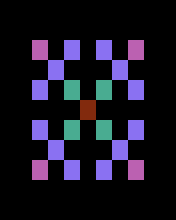
\includegraphics[width=1.3cm]{src/colorspace_patterns/pixels/pixel_pattern5_15.png}%
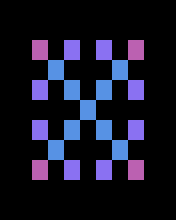
\includegraphics[width=1.3cm]{src/colorspace_patterns/pixels/pixel_pattern5_16.png}%
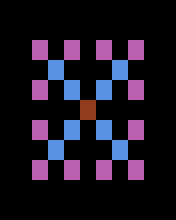
\includegraphics[width=1.3cm]{src/colorspace_patterns/pixels/pixel_pattern5_17.png}%
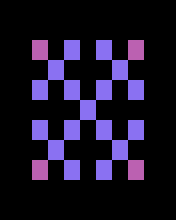
\includegraphics[width=1.3cm]{src/colorspace_patterns/pixels/pixel_pattern5_18.png}%
} \\
        \midrule

        \makecell[l]{
\icode{.BYTE \$FC,\$04,\$04,\$FC}\\
\icode{.BYTE \$FC,\$FC,\$04,\$04}
} & \makecell[l]{
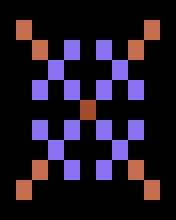
\includegraphics[width=1.3cm]{src/colorspace_patterns/pixels/pixel_pattern5_19.png}%
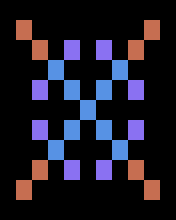
\includegraphics[width=1.3cm]{src/colorspace_patterns/pixels/pixel_pattern5_20.png}%
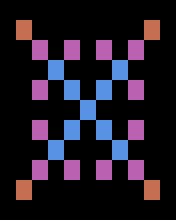
\includegraphics[width=1.3cm]{src/colorspace_patterns/pixels/pixel_pattern5_21.png}%
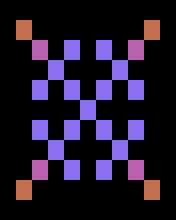
\includegraphics[width=1.3cm]{src/colorspace_patterns/pixels/pixel_pattern5_22.png}%
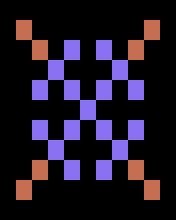
\includegraphics[width=1.3cm]{src/colorspace_patterns/pixels/pixel_pattern5_23.png}%

\includegraphics[width=1.3cm]{src/colorspace_patterns/pixels/pixel_pattern5_24.png}%
} \\
        \midrule

        \makecell[l]{
\icode{.BYTE \$FB,\$FD,\$03,\$05,\$05,\$03,\$FD,\$FB}\\
\icode{.BYTE \$FD,\$FB,\$FB,\$FD,\$03,\$05,\$05,\$03}
} & \makecell[l]{

\includegraphics[width=1.3cm]{src/colorspace_patterns/pixels/pixel_pattern5_25.png}%

\includegraphics[width=1.3cm]{src/colorspace_patterns/pixels/pixel_pattern5_26.png}%

\includegraphics[width=1.3cm]{src/colorspace_patterns/pixels/pixel_pattern5_27.png}%

\includegraphics[width=1.3cm]{src/colorspace_patterns/pixels/pixel_pattern5_28.png}%

\includegraphics[width=1.3cm]{src/colorspace_patterns/pixels/pixel_pattern5_29.png}%

\includegraphics[width=1.3cm]{src/colorspace_patterns/pixels/pixel_pattern5_30.png}%
} \\
        \midrule

          \end{tabular}
        \end{adjustbox}
      }\caption{Pattern Progression for 'Sloth Multi-Cross'}
    \end{figure}
    
